\subsection{Paper prototype test}
\label{sec:paperprototypetest}
In the early stages of development, it might be useful to do a paper prototype test. This test is done by making a prototype of the user interface on paper, 
and having one person (the "computer") change between the different paper screens based on what the user being tested clicks on. 

We did some early paper prototype testing in our project, on the 4th of September. After our workshop we had made some screen layout mockups, see figure \ref{fig:paperprototype}, 
and we wanted to test how user friendly these were.

\begin{figure}
	%\vspace{-4cm}
	%\hspace{4cm}
	\center
		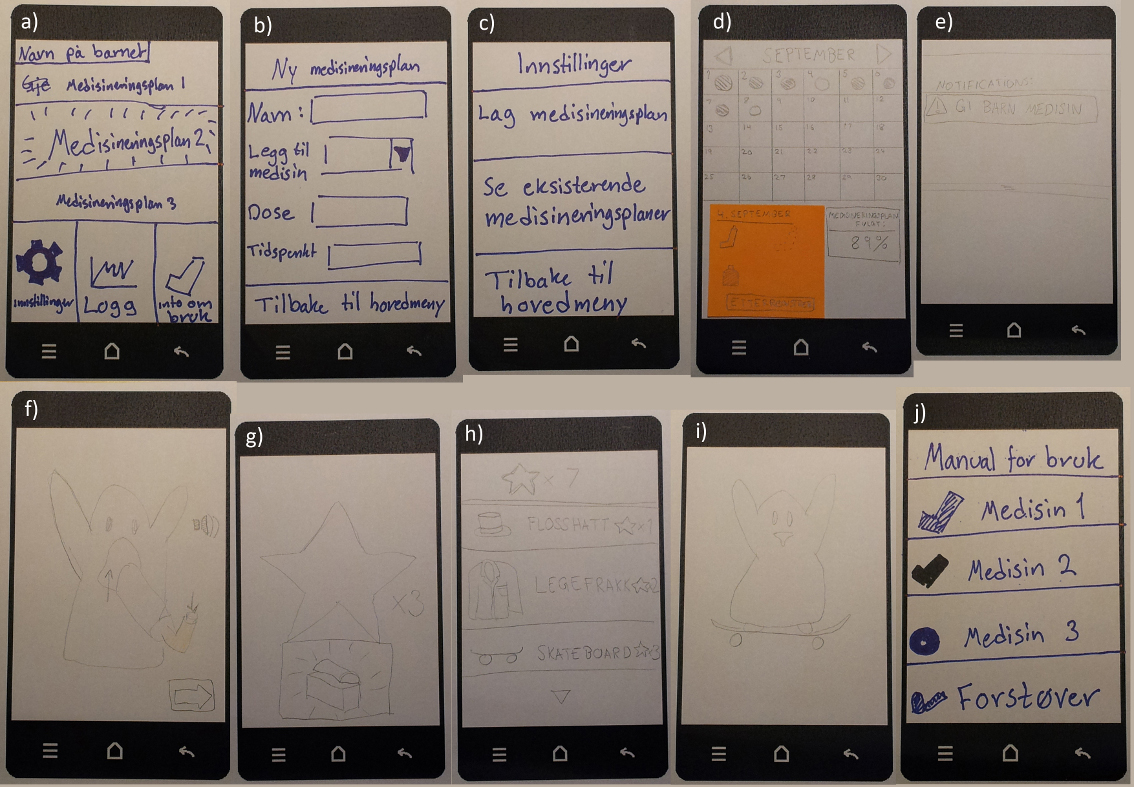
\includegraphics[width=0.8\paperheight, angle=90]{Pictures/PaperprototypeScaled}

	\caption[Paper prototype]{The screens of the paper prototype: a) The GAPP mainscreen. 

								b) GAPP new medication screen.
								c) GAPP settings screen
								d) GAPP log screen.
								e) Notification on phone
								f) One of the CAPP distraction screens.
								g) The CAPP reward screen
								h) CAPP shop screen
								i) CAPP avatar screen, after buying skateboard in the shop
								j) the GAPP manual screen}
	\label{fig:paperprototype}
\end{figure}

The test was done with the expert review method. We had a person from NAAF come for the test, to solve the tasks with the system we provided. We chose to do the expert
review mainly because our funder was interested in seeing how the project was proceeding. NAAF is also the main provider of information such as instructions and 
how the medical plans looks, so having one of them see the system was helpful, as we at this point was uncertain about alot of these things.

From the development group, Eirik and Aleks attended the test. Eirik played the part of the computer, while Aleks introduced the test, explained the system and handled
any other talking that needed to be done.\\
The preconditions we assumed to be present for the CAPP was:
\begin{itemize}
	\item A paper prototype with the correct screens.
	\item Basic knowledge of Android devices in the user being tested.
	\item An active notification for taking medicine on the android device.
\end{itemize}
for GAPP these precondition were:
\begin{itemize}
	\item A paper prototype with the correct screens.
	\item Basic knowledge of android devices in the user being tested.
	\item The correct medication plans and medicines registered in the system.
\end{itemize}

We had prepared a set of tasks for each of our two android applications, CAPP and GAPP. We did not have a functional application for the karotz at this point, and it was difficult to
test this with a paper prototype, so we chose to leave that part out of this test. The cases can be seen in table \ref{tab:capptasks} and table \ref{tab:gapptasks}.

\begin{table}[h]
	\begin{center}
		\begin{tabular}{|p{1.0cm}|p{10.0cm}|}
			\hline
			\bf{Task} & \bf{Description}\\
			\hline
			\bf{1} & There is an active notification for medication on the phone, follow the instructions given by the android device.\\
			\bf{2} & Go to the shop in CAPP and buy a skateboard for the avatar.\\
			\hline
		\end{tabular}
	\end{center}
	\caption{The tasks for CAPP}
	\label{tab:capptasks}
\end{table}

\begin{table}[h]
	\begin{center}
		\begin{tabular}{|p{1.0cm}|p{10.0cm}|}
			\hline
			\bf{Task} & \bf{Description}\\
			\hline
			\bf{1} & Open GAPP.\\
			\bf{2} & Register use of "Medisin 1" on 4th of september.\\
			\bf{3} & Check for more iformation on correct usage of "Medisin 2".\\
			\hline
		\end{tabular}
	\end{center}
	\caption{The tasks for GAPP}
	\label{tab:gapptasks}
\end{table}

This test gave us some strong feedback on what parts of the system worked well, and what didn't make sense at all. We also sat down and had an interview with
the test person after the test regarding the best way to present the information we would get from NAAF.
Some of the problems the test person had might be credited to her being inexperienced with android devices, but we noted down these problems aswell.
 In short the paper prototype test gave us the following results:

\begin{itemize}
	\item Having the reminder as a notification is insufficient. The test person had trouble noticing it even though she was told it would be there.
	\item CAPP have to inform how many times you should press the medicine during medication.
	\item The rewardscreen in CAPP is not intuitive enough.
	\item The main menu in GAPP needs a complete rework, the menu system was not easy to understand.
	\item The Log have to be clearer on how to register medicines, and which medicines is already registered.
	\item There is no back button in the application. This is a problem with android experience, and we didn't implement a back button in the end.
	\item The Information about correct use of medicines was not easily accessible.
\end{itemize} 
The paper prototype led to a major overhaul of the user interface.